%%%%%%%%%%%%%%%%%%%%%%%%%%%%%%%%%%%%%%%%%
% a0poster Portrait Poster
% LaTeX Template
% Version 1.0 (22/06/13)
%
% The a0poster class was created by:
% Gerlinde Kettl and Matthias Weiser (tex@kettl.de)
% 
% This template has been downloaded from:
% http://www.LaTeXTemplates.com
%
% License:
% CC BY-NC-SA 3.0 (http://creativecommons.org/licenses/by-nc-sa/3.0/)
%
%%%%%%%%%%%%%%%%%%%%%%%%%%%%%%%%%%%%%%%%%

%----------------------------------------------------------------------------------------
%	PACKAGES AND OTHER DOCUMENT CONFIGURATIONS
%----------------------------------------------------------------------------------------

\documentclass[40pt, a0, portrait]{a0poster}

\usepackage{multicol} % This is so we can have multiple columns of text side-by-side
\columnsep=100pt % This is the amount of white space between the columns in the poster
\columnseprule=3pt % This is the thickness of the black line between the columns in the poster

\usepackage[svgnames]{xcolor} % Specify colors by their 'svgnames', for a full list of all colors available see here: http://www.latextemplates.com/svgnames-colors

\usepackage{times} % Use the times font
%\usepackage{palatino} % Uncomment to use the Palatino font

\usepackage{graphicx} % Required for including images
\graphicspath{{figures/}} % Location of the graphics files
\usepackage{booktabs} % Top and bottom rules for table
\usepackage[font=small,labelfont=bf]{caption} % Required for specifying captions to tables and figures
\usepackage{amsfonts, amsmath, amsthm, amssymb} % For math fonts, symbols and environments
\usepackage{wrapfig} % Allows wrapping text around tables and figures

\begin{document}

%----------------------------------------------------------------------------------------
%	POSTER HEADER 
%----------------------------------------------------------------------------------------

% The header is divided into two boxes:
% The first is 75% wide and houses the title, subtitle, names, university/organization and contact information
% The second is 25% wide and houses a logo for your university/organization or a photo of you
% The widths of these boxes can be easily edited to accommodate your content as you see fit

\begin{minipage}[b]{0.75\linewidth}
\veryHuge \color{NavyBlue} \textbf{An ontology, artificial inteligence and
frequency-based approach to recommend activities in
scientific workflows} \color{Black}\\ % Title
\\
%\Huge\textit{An Exploration of Complexity}\\[2cm] % Subtitle
\huge \textbf{Adilson Lopes Khouri \& Luciano Antonio Digiampietri}\\[0.5cm] % Author(s)
\huge University of São Paulo EACH\\[0.4cm] % University/organization
\Large \texttt{adilson.khouri.usp@gmail.com} \\
\Large \texttt{luciano.digiampietri@gmail.com}
\end{minipage}
%
\begin{minipage}[b]{0.25\linewidth}

\includegraphics[width=20cm]{usp.png}\\
\end{minipage}

\vspace{1cm} % A bit of extra whitespace between the header and poster content

%----------------------------------------------------------------------------------------

\begin{multicols}{2} % This is how many columns your poster will be broken into, a portrait poster is generally split into 2 columns

%----------------------------------------------------------------------------------------
%	ABSTRACT
%----------------------------------------------------------------------------------------

%\color{Navy} % Navy color for the abstract
%
%\begin{abstract}
%
%The number of activities provided by scientific workflow management systems is large, which requires scientists to know many of them to take advantage of the reusability provided by these systems. To minimize this problem, the literature presents some techniques to recommend activities during the scientific workflow construction. This paper contribution is a hybrid activity recommendation system considering information on frequency, input and outputs of activities and ontological annotations. Additionally, this project presents a modeling of activities recommendation as a classification problem, tested using 5 classifiers; 5 regressors; a SVM classifier, which uses the results of other classifiers and regressors to recommend; and an ensemble of classifiers (Rotation Forest). The proposed technique was compared to other related techniques and to classifiers and regressors, using 10-fold-cross-validation, achieving a MRR at least 70\% greater than those obtained by other techniques.
%
%
%\end{abstract}

%----------------------------------------------------------------------------------------
%	INTRODUCTION
%----------------------------------------------------------------------------------------

\color{Navy} % SaddleBrown color for the introduction

\section*{Introduction}

The number of research projects using intensive computing has been growing in areas that lack advanced computer skills such as biology, physics, and astronomy. One of the tools to assist in the management and construction of intensive computing experiments are the workflows manager systems. \emph{Scientific Workflows} represent structured and ordered processes, constructed manually, semi-automatically or automatically to solve scientific problems using activities, which can be: i) source code blocks; (ii) services; or iii) finished workflows \cite{Wang2010}. These systems facilitate the creation of new experiments, sharing of results and reuse of existing activities.

Nowadays, there are a large number of activities available in repositories such as \emph{myExperiment} which stores more than 2,500 workflows\footnote{http://www.myexperiment.org/} and \emph{BioCatalogue} Which provides more than 2,464 services~\cite{Biocatalogue}. The large number of activities and the low reuse of some activities and workflows motivate the construction of techniques to recommend activities to the scientists during the composition of workflows~\cite{Wang2010}.

In the workflow management systems, activities are typically represented as graphical icons with drag and drop functionality. Thus, it is possible to construct computational experiments by dragging icons and filling in input parameters. Most of these systems provide sets of basic activities that can be used in different domains, for example, an activity that calculates the average value of a set of data is applicable in biology, physics, astronomy, and other areas. However, there is a precondition for reusing and\/or creating workflows: knowing the available activities.

In order to minimize the problem of knowing a large number of activities, several techniques were proposed to recommend activities or to compose workflows. In the first case, which aims to serve an expert user in these systems, during the construction of the workflow, activities are recommended to help to complete the workflow. In the second case, whose goal is to serve a less expert user on these systems, several workflows are built and the user should select which one most satisfies him\/her need.

This paper presents a hybrid approach for recommending activities in scientific workflows based on the frequency of activities combined with a knowledge-base ontology for data sets without provenance information, and without reliability data about the authors of the services and workflows. We also propose a modeling of the problem of recommending activities in scientific workflows to be used by classifiers such as: Support Vector Machine (SVM), Naive Bayes (NB), K-Nearest-Neighbor (KNN), Classification and Regression Trees, and Neural Network (MLP). The following regressors were also used: Support Vector Regression (SVR), CART, Neural Network, Multivariate Adaptive Regression Splines (MARS) and Binomial Regression (RB). At last, a comparison of our approach and the approaches from the related literature is presented.

%----------------------------------------------------------------------------------------
%	OBJECTIVES
%----------------------------------------------------------------------------------------

\color{DarkSlateGray} % DarkSlateGray color for the rest of the content

\section*{Main Objectives}

The 73 bioinformatics' workflows together with their 280 activities were converted into a matrix $M_{i, j}$. In this matrix, each line corresponds to a workflow and each column to an activity. $M_{i, j} = 1$ means that the workflows \emph{i} has the activity \emph{j}. Otherwise, $M_{i, j} = 0$ means that the workflow \emph{i} does not have the activity \emph{j}. Table~\ref{tabela_matriz_de_dados} presents an fictitious example of a matrix \(M\). To perform the evaluation of the approach, an activity is removed from each row of the table \ref{tabela_matriz_de_dados}, and a list of possible activities is recommended. The goal of the recommendation system is to correctly identify which activity is missing in the workflow (i.e., the one that was removed).
\begin{center}\vspace{1cm}
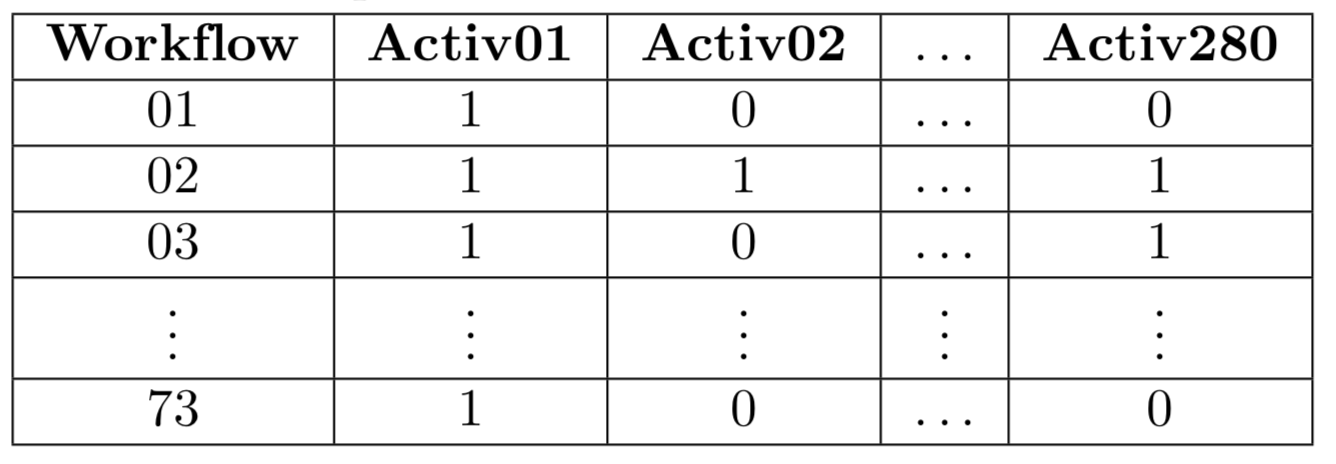
\includegraphics[width=0.8\linewidth]{matrizSimples.png}
\captionof{figure}{\color{Green} Figure caption}
\end{center}\vspace{1cm}

%\begin{table}[htb]
%	\centering
%	\caption{Input matrix example.}
%	\begin{tabular}{|c|c|c|c|c|}  \hline
%		\textbf{Workflow} & \textbf{Activ\(\mathbf{01}\)} & \textbf{Activ\(\mathbf{02}\)} & \textbf{\(\mathbf{\ldots}\)} & \textbf{Activ\(\mathbf{280}\)}  \\ \hline
%		01 			  & 1 			  & 0 			  & \(\ldots\) 	  & 0  				\\ \hline
%		02 			  & 1 			  & 1 			  & \(\ldots\) 	  & 1  				\\ \hline
%		03 			  & 1 			  & 0 			  & \(\ldots\) 	  & 1  				\\ \hline
%		\(\vdots\) 		  			  & \(\vdots\) 	  & \(\vdots\) 	  & \(\vdots\) 	  & \(\vdots\) 		\\ \hline
%		73 			  & 1 			  & 0 			  & \(\ldots\) 	  & 0  				\\ \hline
%	\end{tabular}
%	\label{tabela_matriz_de_dados}
%	\vspace{0.1cm}
%\end{table}

In order to use classification and regression techniques, some changes were proposed in the original dataset (exemplified in the table~\ref{tabela_matriz_de_dados}), which can be viewed in the table~\ref{tabela_matriz_de_dados_adapatada_classificacao_regressao}. Each workflow was replicated \(118\) times. 59 of these correspond to identical copies of the original workflow, while in the other \(59\) one activity was removed from original workflow and a new activity was added representing a possible recommendation. Thus, for each original workflow, there will be \(59\) correct instances and \(59\) incorrect instances and this type of information will be used to train the classifiers or regressors.


\begin{center}\vspace{1cm}
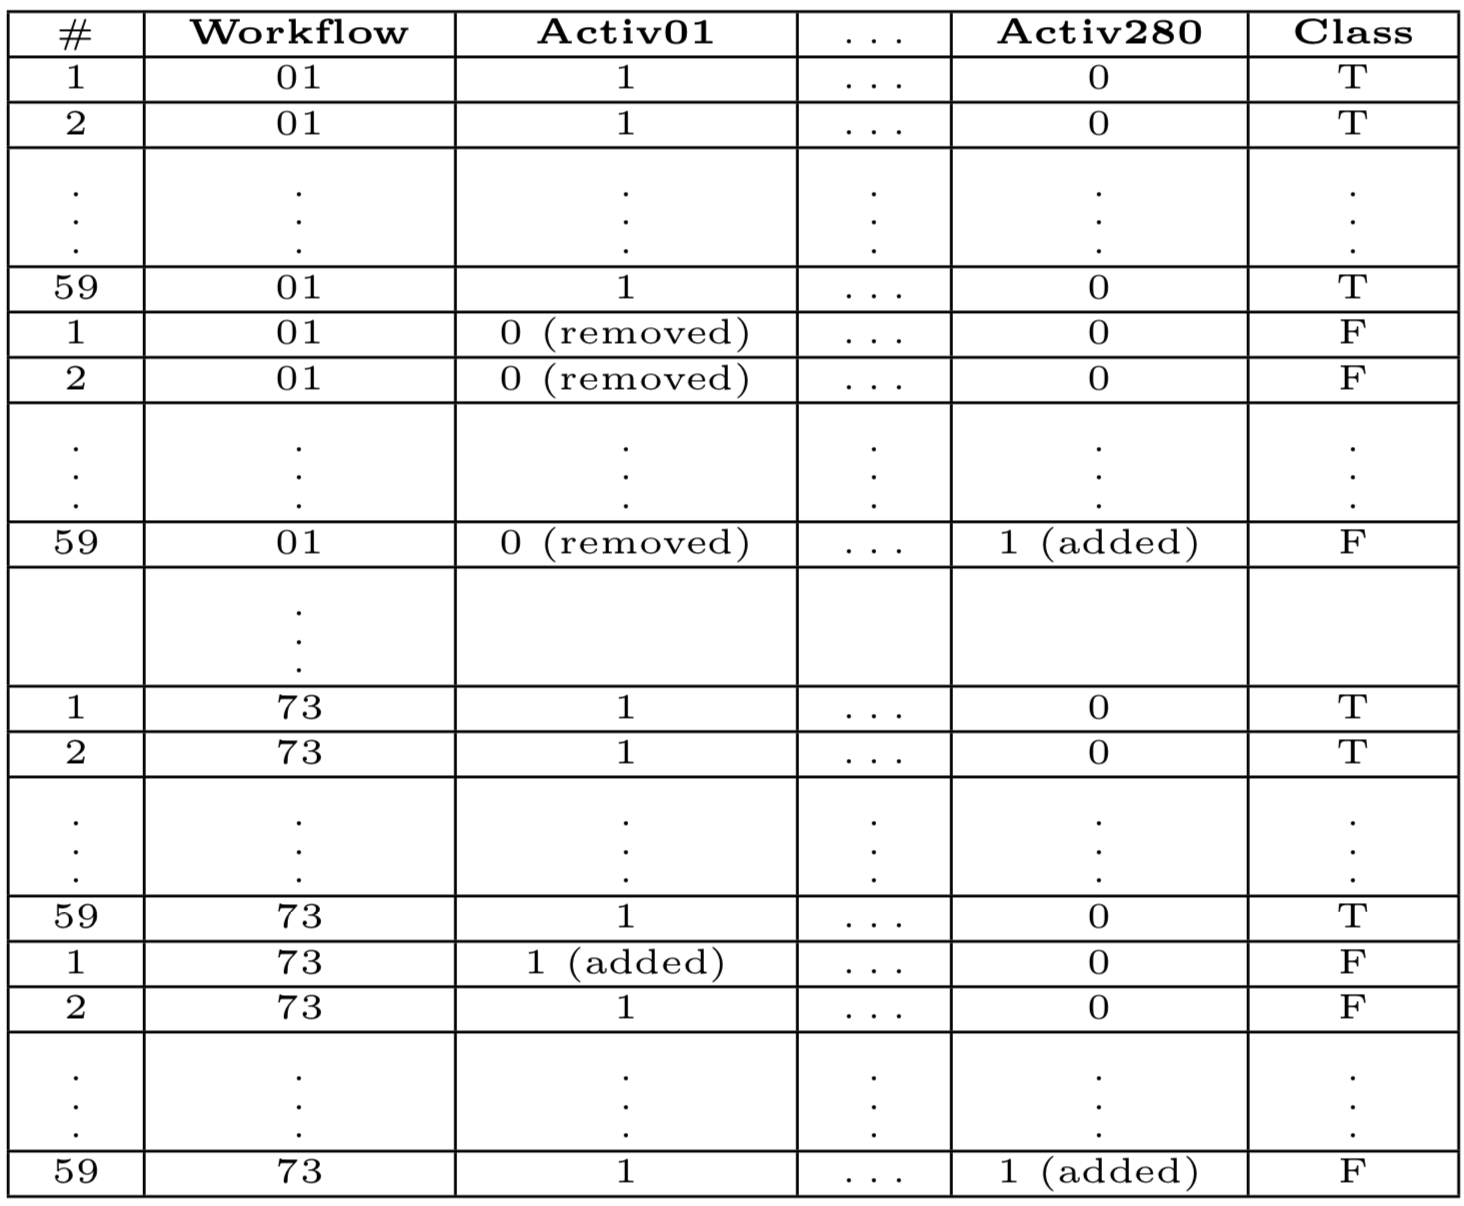
\includegraphics[width=0.8\linewidth]{matrizAdaptada.png}
\captionof{figure}{\color{Green} Figure caption}
\end{center}\vspace{1cm}

%\begin{table}[!htb]
%%	\tiny
%%	\centering
%	\caption{Input matrix used by classifiers and regressors}
%	\begin{tabular}{|c|c|c|c|c|c|c|c|c|}  \hline
%		\textbf{\(\#\)} & \textbf{Workflow} & \textbf{Activ\(\mathbf{01}\)} & \textbf{Activ\(\mathbf{02}\)} & \textbf{\(\mathbf{\ldots}\)}  & \textbf{Activ\(\mathbf{279}\)} & \textbf{Activ\(\mathbf{280}\)} & \textbf{Class} \\ \hline
%		
%		1	&		01		 			   & 1 			  & 0 			  & \(\ldots\) 	  & 0 & 0  			& T	\\ \hline
%		2	&		01 					   & 1 			  & 0 			  & \(\ldots\) 	  & 0 & 0  			& T	\\ \hline
%		\(\vdots\)  &  \(\vdots\) 	   	   & \(\vdots\)   & \(\vdots\) 	  & \(\vdots\) 	  & \(\vdots\) & \(\vdots\) & \(\vdots\)\\ \hline
%		59	&		01 					   & 1 			  & 0 			  & \(\ldots\) 	  & 0 & 0   		& T	\\ \hline
%		1	&		01		 			   & 0 (removed) 		  & 1 (added) &\(\ldots\)& 1 & 0	& F	\\ \hline
%		2	&		01 					   & 0 (removed)& 0 		  & \(\ldots\) 	  & 1 (added) & 0& F	\\ \hline
%		\(\vdots\)  &		\(\vdots\) 	   & \(\vdots\) & \(\vdots\) 	  & \(\vdots\) 	  & \(\vdots\) & \(\vdots\) & \(\vdots\) \\ \hline
%		59	&		01 					   & 0 (removed)			  & 0 			  & \(\ldots\) & 0 & 1 (added)& F \\ \hline
%		&\(\vdots\) & & & & & & 																		\\ \hline
%		1	&		73		 			   & 1 			  & 1  & \(\ldots\) 	  & 0 & 0  			& T	\\ \hline
%		2	&		73 					   & 1 			  & 1  & \(\ldots\) 	  & 0 & 0  			& T	\\ \hline
%		\(\vdots\)  &		\(\vdots\) 	   & \(\vdots\)   & \(\vdots\) 	  & \(\vdots\) 	  & \(\vdots\) & \(\vdots\) & \(\vdots\) \\ \hline
%		59	&		73 					   & 1 			  & 1  & \(\ldots\) 	  & 0 & 0   		& T	\\ \hline
%		1	&		73		 			   & 1 (added) & 0 (removed)  & \(\ldots\) 	  & 1 & 0   		& F	\\ \hline
%		2	&		73 					   & 1 			  & 0 (removed)  & \(\ldots\)& 1 (added) & 0  & F	\\ \hline
%		\(\vdots\)  &		\(\vdots\) 	   & \(\vdots\)   & \(\vdots\) 	  & \(\vdots\) 	  & \(\vdots\) & \(\vdots\) & \(\vdots\)	\\ \hline
%		59	&		73 					   & 1 			  & 0 (removed)  & \(\ldots\) 	  & 0 & 1 (added) & F	\\ \hline
%	\end{tabular}
%	\label{tabela_matriz_de_dados_adapatada_classificacao_regressao}
%	\vspace{0.1cm}
%	%\source{\varAutorData}
%\end{table}

%----------------------------------------------------------------------------------------
%	RESULTS 
%----------------------------------------------------------------------------------------

\section*{Results}

\begin{center}\vspace{1cm}
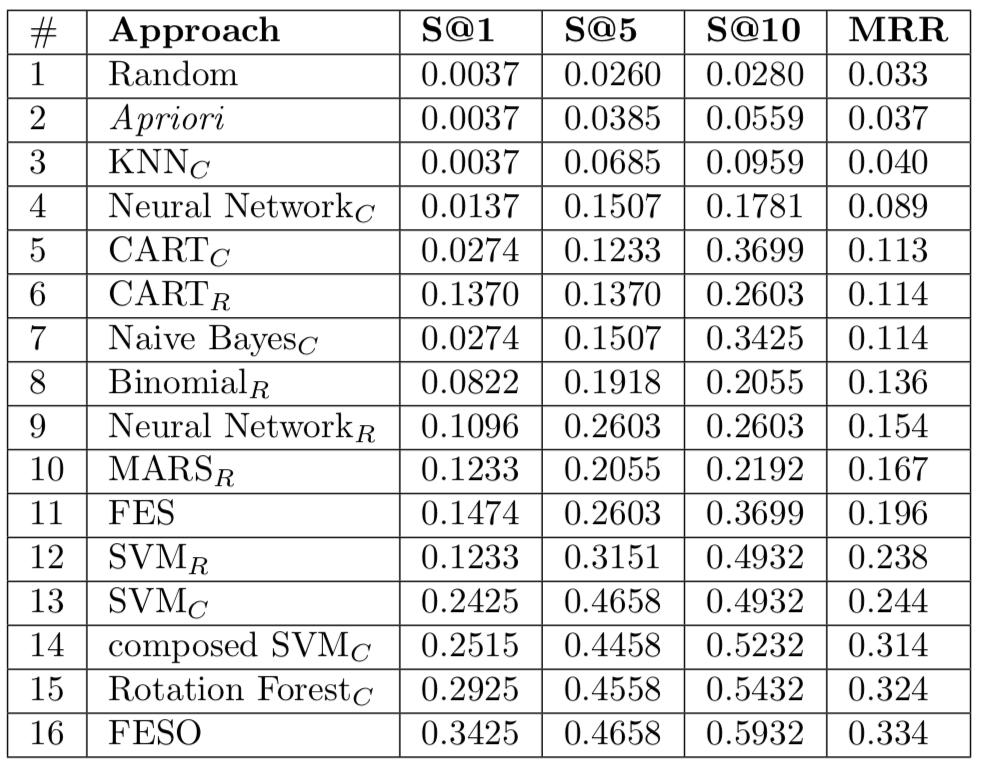
\includegraphics[width=0.8\linewidth]{resultados.png}
\captionof{figure}{\color{Green} Figure caption}
\end{center}\vspace{1cm}

%Donec faucibus purus at tortor egestas eu fermentum dolor facilisis. Maecenas tempor dui eu neque fringilla rutrum. Mauris \emph{lobortis} nisl accumsan. Aenean vitae risus ante.
%%
%\begin{wraptable}{l}{12cm} % Left or right alignment is specified in the first bracket, the width of the table is in the second
%\begin{tabular}{l l l}
%\toprule
%\textbf{Treatments} & \textbf{Response 1} & \textbf{Response 2}\\
%\midrule
%Treatment 1 & 0.0003262 & 0.562 \\
%Treatment 2 & 0.0015681 & 0.910 \\
%Treatment 3 & 0.0009271 & 0.296 \\
%\bottomrule
%\end{tabular}
%\captionof{table}{\color{Green} Table caption}
%\end{wraptable}
%%
%Phasellus imperdiet, tortor vitae congue bibendum, felis enim sagittis lorem, et volutpat ante orci sagittis mi. Morbi rutrum laoreet semper. Morbi accumsan enim nec tortor consectetur non commodo nisi sollicitudin. Proin sollicitudin. Pellentesque eget orci eros. Fusce ultricies, tellus et pellentesque fringilla, ante massa luctus libero, quis tristique purus urna nec nibh.
%
%Nulla ut porttitor enim. Suspendisse venenatis dui eget eros gravida tempor. Mauris feugiat elit et augue placerat ultrices. Morbi accumsan enim nec tortor consectetur non commodo. Pellentesque condimentum dui. Etiam sagittis purus non tellus tempor volutpat. Donec et dui non massa tristique adipiscing. Quisque vestibulum eros eu. Phasellus imperdiet, tortor vitae congue bibendum, felis enim sagittis lorem, et volutpat ante orci sagittis mi. Morbi rutrum laoreet semper. Morbi accumsan enim nec tortor consectetur non commodo nisi sollicitudin.
%
%\begin{center}\vspace{1cm}
%
\includegraphics[width=0.8\linewidth]{placeholder}
%\captionof{figure}{\color{Green} Figure caption}
%\end{center}\vspace{1cm}
%
%In hac habitasse platea dictumst. Etiam placerat, risus ac.
%
%Adipiscing lectus in magna blandit:
%
%\begin{center}\vspace{1cm}
%\begin{tabular}{l l l l}
%\toprule
%\textbf{Treatments} & \textbf{Response 1} & \textbf{Response 2} \\
%\midrule
%Treatment 1 & 0.0003262 & 0.562 \\
%Treatment 2 & 0.0015681 & 0.910 \\
%Treatment 3 & 0.0009271 & 0.296 \\
%\bottomrule
%\end{tabular}
%\captionof{table}{\color{Green} Table caption}
%\end{center}\vspace{1cm}
%
%Vivamus sed nibh ac metus tristique tristique a vitae ante. Sed lobortis mi ut arcu fringilla et adipiscing ligula rutrum. Aenean turpis velit, placerat eget tincidunt nec, ornare in nisl. In placerat.
%
%\begin{center}\vspace{1cm}
%
\includegraphics[width=0.8\linewidth]{placeholder}
%\captionof{figure}{\color{Green} Figure caption}
%\end{center}\vspace{1cm}

%----------------------------------------------------------------------------------------
%	CONCLUSIONS
%----------------------------------------------------------------------------------------

\color{SaddleBrown} % SaddleBrown color for the conclusions to make them stand out

\section*{Conclusions}

\begin{itemize}
\item This work developed a hybrid technique for recommending activities in scientific workflows, which uses syntactic compatibility, frequency, and domain ontologies to recommend activities, called FESO
\item The developed technique is better than every other technique from literature
\item We have modeled the recommendation problem as a regression and classification problem in artificial intelligence
\item The main idea of the project was to add structured semantic information to the recommendation system
\item The activities were not independent
\item The problem is not linearly separable
\end{itemize}

\color{DarkSlateGray} % Set the color back to DarkSlateGray for the rest of the content

%----------------------------------------------------------------------------------------
%	FORTHCOMING RESEARCH
%----------------------------------------------------------------------------------------

\section*{Forthcoming Research}

Vivamus molestie, risus tempor vehicula mattis, libero arcu volutpat purus, sed blandit sem nibh eget turpis. Maecenas rutrum dui blandit lorem vulputate gravida. Praesent venenatis mi vel lorem tempor at varius diam sagittis. Nam eu leo id turpis interdum luctus a sed augue. Nam tellus.

 %----------------------------------------------------------------------------------------
%	REFERENCES
%----------------------------------------------------------------------------------------

\nocite{*} % Print all references regardless of whether they were cited in the poster or not
\bibliographystyle{plain} % Plain referencing style
\bibliography{sample} % Use the example bibliography file sample.bib

%----------------------------------------------------------------------------------------
%	ACKNOWLEDGEMENTS
%----------------------------------------------------------------------------------------

\section*{Acknowledgements}

We thank the University of São Paulo (USP) and the CAPES agency wich provided scholarships for the student. Allowing to complete this master with publications in the area of computer science.

%----------------------------------------------------------------------------------------

\end{multicols}
\end{document}